% Dies ist Teil der Vorlesung Physik auf dem Computer, SS 2012,
% Axel Arnold, Universitaet Stuttgart.
% 
% Dieses Werk ist unter einer Creative Commons-Lizenz vom Typ
% Namensnennung-Weitergabe unter gleichen Bedingungen 3.0 Deutschland
% zugänglich. Um eine Kopie dieser Lizenz einzusehen, konsultieren Sie
% http://creativecommons.org/licenses/by-sa/3.0/de/ oder wenden Sie sich
% schriftlich an Creative Commons, 444 Castro Street, Suite 900, Mountain
% View, California, 94041, USA.

\chapter{Numerisches Differenzieren und Integrieren}

In diesem Kapitel geht es darum, wie eine Funktion, die an diskreten
Stützstellen gegeben ist, numerisch differenziert und integriert
werden kann. Die Grundlagen dazu wurden bereits mit dem Kapitel
``Darstellung von Funktionen'' gelegt, denn das interpolierende
Polynom oder auch ein Spline lassen sich ja auch mit dem Computer
leicht analytisch integrieren.

\section{Numerisches Differenzieren}

Die erste Ableitung einer Funktion $f\in C^1([a,b])$ ist definiert als
\begin{equation}
  \lim_{h\to 0} \frac{f(x+h) - f(x)}{h}.
\end{equation}
Ist $f$ nun nur an diskreten Punkten bekannt, so liegt es nahe, die
Ableitung durch die dividierte Differenz
\begin{equation}
  f' \approx f[x,y] := \frac{f(x) - f(y)}{x - y}
\end{equation}
anzunähern, wobei $x$ und $y$ nahe beieinander liegen sollten.

Doch an welchem Punkt ist diese Näherung optimal? Gemäß Mittelwertsatz
gilt auf jeden Fall $f[x,y]=f'(\xi)$ für ein $\xi\in [x,y]$. Es liegt
nahe, anzunehmen, dass $f[x,y]$ am besten in der Intervalmitte
$m=\frac{x+y}{2}$ approximiert. Das ist tatsächlich so, wie wir nun
per Taylorentwicklung sehen werden. Mit Entwicklung um $m$ und $h=x-y$
gilt
\begin{align}
  \frac{f(x) - f(y)}{x-y} &= \frac{1}{h}
  \biggl(+f(m) + \frac{h}{2}f'(m) + \frac{h^2}{8}f''(m) + \O(h^3)\nonumber\\
  &\phantom{= \frac{1}{h}\biggl(}-f(m) + \frac{h}{2}f'(m) - \frac{h^2}{8}f''(m) + \O(h^3)
  \biggr)\nonumber\\
  &=  f'(m) + \O(h^2).
\end{align}
Bei Ansatzpunkt $x$ gilt hingegen nur
\begin{align}
  \frac{f(x) - f(y)}{x-y} = \frac{1}{h}
  \biggl(f(x) + h f'(x) + \frac{h^2}{8}f''(x) + \O(h^3) - f(x) \biggr)
  =  f'(x) + \O(h).
\end{align}

In der Praxis ist die Funktion meist an an äquidistanten Stützstellen
$x_i$ mit $x_{i+1}-x_i=h$ gegeben. Dann ist, wie oben gezeigt, die
beste Zweipunkt-Näherung für die Ableitung die zentrale Differenz
\begin{equation}
  f[x_{i-1},x_{i+1}] = f'(x_i) + \O(h^2),
\end{equation}
während für die linken und rechten dividierten Differenzen gilt:
\begin{equation}
  f[x_{i},x_{i+1}] = f'(x_i) + \O(h) =  f[x_{i-1},x_{i}].
\end{equation}

\subsection{Näherungen höhererer Ordnung und höhere Ableitungen}

Mit Hilfe von Taylorentwicklungen lassen sich auch Näherungen mit mehr
Stützpunkten und für höhere Ableitungen entwickeln.  Wir betrachten
zum Beispiel die Punkte für $k=-2(1)2$, d.h. die 5 benachbarten
Punkte, und suchen Koeffizienten $c_k$ derart, dass
\begin{equation}
  c_2 f(x_{i+2}) + c_1 f(x_{i+1})  + c_0 f(x_i) + c_{-1}f(x_{i-1}) +
  c_{-2}f(x_{i-2}) = f'(x_i) + \O(h^5),
\end{equation}
unabhänging von der Form von $f$ und seiner Ableitungen.  Durch
Einsetzen der Taylorentwicklung
\begin{equation}
  f(x + k h) = f(x) + k\, hf'(x) + k^2\,\frac{h^2}{2} f''(x_i) +
  k^3\,\frac{h^3}{6}f^{(3)}(x) + k^4\,\frac{h^4}{24}f^{(4)}(x) + \O(h^5)
\end{equation}
folgt dann, in der Reihenfolge der Ableitungen in der Taylorentwicklung
\begin{align}
  \label{eq:derivatives}
  c_{2} + c_{-2} + c_{-1} + c_1 + c_0 &= 0\nonumber\\
  h\left[2 (c_{2} - c_{-2})  + c_{1} - c_{-1}\right] &= 1\nonumber\\
  \frac{h^2}{2}\left[4(c_{2} + c_{-2})  + c_{1} + c_{-1}\right] &= 0\nonumber\\
  \frac{h^3}{6}\left[8 (c_{2} - c_{-2})  + c_{1} - c_{-1}\right] &= 0\nonumber\\
  \frac{h^4}{24}\left[16 (c_{2} + c_{-2}) + c_{1} + c_{-1}\right] &= 0.
\end{align}
Durch Lösen des Gleichungssystems folgt
\begin{equation}
  \label{eq:5orderdiff}
  -\frac{1}{12h} f(x_{i+2}) + \frac{2}{3h} f(x_{i+1})  - \frac{2}{3h} f(x_{i-1}) +
  \frac{1}{12h}f(x_{i-2}) = f'(x_i) + \O(h^4).
\end{equation}
Auf diese Weise lässt sich auch die höhere Güte der zentralen
Differenz verstehen: tatsächlich entspricht diese der optimalen
Näherung durch $x_{i-1}$, $x_i$  und $x_{i+1}$, nur dass aus
Symmetriegründen der Koeffizient zu $x_i$ verschwindet.

Um nun zum Beispiel die zweite Ableitung zu berechnen, lösen wir
\eqref{eq:derivatives}, allerdings mit einer 1 nicht in der zweiten,
sondern dritten Zeile. Das ergibt
\begin{equation}
  \frac{1}{h^2}\left(-\frac{1}{12} f(x_{i+2}) + \frac{4}{3} f(x_{i+1}) +
  \frac{5}{2} f(x_i)  + \frac{4}{3} f(x_{i-1}) -
  \frac{1}{12}f(x_{i-2})\right) = f''(x_i) + \O(h^3).
\end{equation}

Mit drei Stützpunkten ergibt sich die Näherung für die zweite
Ableitung analog als
\begin{multline}
  \frac{1}{h^2}\bigl(f(x_{i+1}) -
  2f(x_i)  + f(x_{i-1})\bigr) =
  \frac{\frac{f(x_{i+1}) - f(x_i)}{h}  -
    \frac{f(x_i) - f(x_{i-1})}{h}}{h}
  = f''(x_i) + \O(h).
\end{multline}
Die mittlere Form zeigt, dass sich diese einfachste Form der zweiten
Ableitung auch als dividierte Differenz der dividierten Differenzen
verstehen lässt. Technisch wird also die zweite Ableitung also einfach
in erster Ordnung aus der ersten Ableitung in erster Ordnung
bestimmt. Analog lässt sich jede $n$-te Ableitung aus $n+1$
benachbarten Stützstellen in erster Ordnung durch dividierte
Differenzen approximieren.
\begin{figure}
  \centering
  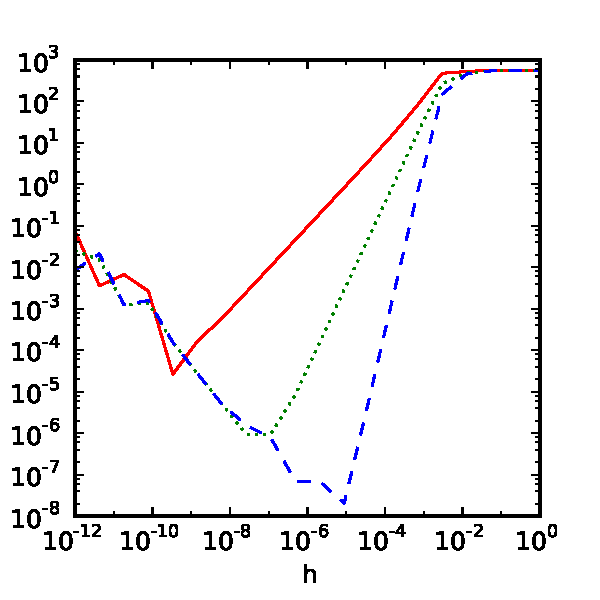
\includegraphics[width=0.5\textwidth]{plots/num_diff}
  \caption{Maximale Abweichung $\max_{x\in[-\pi,pi]} \abs{f'(x) - a(h;
      x)}$ für verschiedene Näherungen $a(h; x)$, als Funktion der
    Schrittweite $h$. Die Funktion ist $f(x)=sin(100*x^2)$. Rot
    durchgezogen ist die linksseitige Differenz $a(h; x) = (f(x) -
    f(x-h))/h$, die zentrale Differenz $a(h; x) = (f(x+h) -
    f(x-h))/2h$ ist grün gepunktet und die Näherung 4. Ordnung
    \eqref{eq:5orderdiff} blau gestrichelt. Der rechtsseitige Abfall
    der Kurven entspricht den Ordnungen $\O(h)$ für die linksseitige
    Differenz, $\O(h^2)$ für die rechtsseitige und $\O(h^4)$ für die
    Gleichung 4. Ordnung. Das linksseitige Verhalten ist
    methodenunabhängig und durch die endliche Rechenauflösung bestimmt.}
  \label{fig:num_diff}
\end{figure}

\subsection{Genauigkeit}

Generell sind alle diese Näherungen numerisch instabil, da bei kleinen
Abständen $h$ auch $f(x)$ und $f(x+h)$ sehr ähnlich sind. Sind diese
betragsmäßig groß, kommt es zu Auslöschung, d.h., $f(x+h) - f(x)$ hat
deutlich weniger signifikante Stellen als Maschinengenauigkeit. Daher
gibt es stets ein optimales $h$, das allerdings von der unbekannten
zweiten Ableitung der betrachteten Funktion abhängt.

Auch Verfahren höherer Ordnung sind nicht notwendigerweise genauer, da
bei manchen Funktionen die Ableitungen sehr rasch wachsen. Dann ist
zwar $h^4$ sehr viel kleiner als $h^2$, aber der Vorfaktor
kompensiert das zunächst. Abbildung~\ref{fig:num_diff} illustriert
dieses Verhalten am Beispiel der Funktion $\sin(100*x^2)$. Erst, wenn
die Schrittweite $h$ unter die charakteristische Breite von etwa 600
sinkt, spielt die Ordnung des Verfahrens eine Rolle. Wird allerdings
$h$ zu klein, zeigt sich die endliche Auflösung, mit der der Rechner
arbeitet, und der Fehler steigt wieder an.

%%% Local Variables: 
%%% mode: latex
%%% TeX-master: "padc.tex"
%%% TeX-PDF-mode: t
%%% End: 
